% !TEX program = pdflatex
% !TEX encoding = UTF-8 Unicode
% =====================================================================
%  DIY Holter ECG — documento conclusivo (sorgente LaTeX, da lavorare a mano)
% ---------------------------------------------------------------------
%  COME E' FATTO:
%   - Il TESTO sta qui sotto: modificalo liberamente, e' tuo.
%   - Le FIGURE sono in  figs/*.png  e le TABELLE + i numeri aggregati
%     stanno in  tables.tex : entrambi si RIGENERANO dai dati con
%         python3 host/dashboard.py        (ricalcola -> HTML + figure)
%         python3 host/export_latex.py     (HTML -> figs/ + tables.tex)
%     quindi non toccarli a mano: aggiungi una registrazione, rilanci i
%     due comandi, e qui cambiano numeri/figure senza perdere il testo.
%   - COMPILA con:  latexmk -pdf holter_report.tex   (o  pdflatex x2)
% =====================================================================
\documentclass[11pt,a4paper]{article}

% ---- font & codifica (newpx = Palatino, taglio editoriale) ----
\usepackage[T1]{fontenc}
\usepackage[utf8]{inputenc}
\usepackage{newtxtext,newtxmath}   % Times (stile paper accademico)
\usepackage{microtype}

% ---- impaginazione ----
\usepackage[a4paper,margin=2.5cm]{geometry}
\usepackage{graphicx}
\graphicspath{{figs/}{figs_manual/}}   % figs/=auto (export_latex.py)  ·  figs_manual/=figure curate a mano
\usepackage{float}
\usepackage{booktabs}
\usepackage{array}
\usepackage{changepage}   % adjustwidth: blocchi rientrati (abstract/disclaimer)
\usepackage{comment}      % \begin{comment}...\end{comment} per escludere blocchi
\usepackage[table,dvipsnames]{xcolor}
\usepackage{enumitem}
\usepackage{caption}
\usepackage{titlesec}
\usepackage{fancyhdr}
\usepackage[hidelinks]{hyperref}

\setlist{nosep,leftmargin=1.6em}
% stile accademico: rientro di prima riga, nessuno spazio tra paragrafi
\setlength{\parindent}{1.4em}
\setlength{\parskip}{0pt}
\linespread{1.05}

% ---- colori ----
\definecolor{accent}{HTML}{7A3B2E}
\definecolor{muted}{HTML}{6B6862}
\definecolor{cInterp}{HTML}{1F7FB0}   % interpolate (silenziose)
\definecolor{cComp}{HTML}{C0392B}     % compensate (sentite)
\definecolor{cCoupled}{HTML}{9A7D0A}  % coupled
\newcommand{\interp}[1]{\textcolor{cInterp}{#1}}
\newcommand{\comp}[1]{\textcolor{cComp}{#1}}
\newcommand{\coupled}[1]{\textcolor{cCoupled}{#1}}
\newcommand{\rrpre}{RR\textsubscript{pre}}
\newcommand{\rrpost}{RR\textsubscript{post}}

% ---- titoli di sezione (numero in accento + filetto) ----
\titleformat{\section}{\normalfont\large\bfseries}{\thesection.}{0.6em}{}
\titleformat{\subsection}{\normalfont\normalsize\bfseries}{\thesubsection}{0.6em}{}
\titlespacing*{\section}{0pt}{2.2ex plus .3ex}{1.0ex}
\titlespacing*{\subsection}{0pt}{1.4ex plus .2ex}{0.6ex}

% ---- didascalie ----
\captionsetup{font={footnotesize,it},labelfont={bf,up},labelsep=period,skip=5pt,justification=justified,singlelinecheck=false}

% ---- testatina ----
\pagestyle{plain}   % numero pagina centrato in basso, stile paper

% ---- scorciatoia figura: \reportfig[width]{file}{didascalia} ----
\newcommand{\reportfig}[3][\linewidth]{%
  \begin{figure}[H]\centering
    \includegraphics[width=#1]{#2}\caption{#3}
  \end{figure}}
% variante per figure grandi: pagina dedicata (float [p]), evita pagine mezze vuote
\newcommand{\reportfigP}[3][\linewidth]{%
  \begin{figure}[p]\centering
    \includegraphics[width=#1]{#2}\caption{#3}
  \end{figure}}

% numeri aggregati + tabelle (AUTO-generati: non modificare a mano)
% Generato da host/export_latex.py - NON modificare a mano.
% Numeri + tabelle si rigenerano dai dati; il testo sta in holter_report.tex

% --- numeri aggregati (snapshot dei dati correnti) ---
\newcommand{\nSessions}{10}
\newcommand{\totMinutes}{894}
\newcommand{\totBeats}{64,974}
\newcommand{\totPVC}{17,288}
\newcommand{\cumBurden}{26.6\%}
\newcommand{\exclMinutes}{45.1 min}
\newcommand{\pauseValley}{1.00}
\newcommand{\pctInterp}{30}
\newcommand{\pctComp}{70}
\newcommand{\methodBeats}{16,970}

% --- tabelle ---
\newcommand{\tableSessions}{%
\begin{center}
\setlength{\tabcolsep}{5pt}\renewcommand{\arraystretch}{1.12}
\footnotesize
\begin{tabular}{lrrrrr}
\toprule
\textbf{Date / time} & \textbf{Duration} & \textbf{N beats} & \textbf{PVC} & \textbf{Burden} & \textbf{Excluded} \\
\midrule
2026-06-05 14:59 & 14.5 min & 647 & 272 & 29.6\% & 7 (136s) \\
2026-06-05 18:29 & 19.4 min & 1,041 & 341 & 24.7\% & 1 (2s) \\
2026-06-06 13:41 & 53.6 min & 2,453 & 924 & 27.4\% & 32 (537s) \\
2026-06-06 15:08 & 50.5 min & 2,869 & 750 & 20.7\% & 4 (6s) \\
2026-06-07 11:33 & 29.7 min & 1,470 & 697 & 32.2\% & 13 (43s) \\
2026-06-07 21:22 & 214.0 min & 10,031 & 4,851 & 32.6\% & 36 (836s) \\
2026-06-08 22:01 & 247.7 min & 12,324 & 5,168 & 29.5\% & 36 (840s) \\
2026-06-09 13:23 & 70.4 min & 5,330 & 600 & 10.1\% & 4 (41s) \\
2026-06-09 16:58 & 112.5 min & 6,570 & 2,227 & 25.3\% & 8 (195s) \\
2026-06-09 20:54 & 81.6 min & 4,951 & 1,458 & 22.7\% & 6 (68s) \\
\bottomrule
\end{tabular}
\end{center}
}

\newcommand{\tableOutlier}{%
\begin{center}
\setlength{\tabcolsep}{5pt}\renewcommand{\arraystretch}{1.12}
\footnotesize
\begin{tabular}{lr}
\toprule
\textbf{Session} & \textbf{Mean r} \\
\midrule
2026-06-09 13:23 & 0.962 \\
2026-06-05 14:59 & 0.973 \\
2026-06-05 18:29 & 0.977 \\
2026-06-06 15:08 & 0.979 \\
2026-06-09 20:54 & 0.979 \\
2026-06-07 21:22 & 0.980 \\
2026-06-09 16:58 & 0.982 \\
2026-06-08 22:01 & 0.983 \\
2026-06-07 11:33 & 0.984 \\
2026-06-06 13:41 & 0.986 \\
\bottomrule
\end{tabular}
\end{center}
}

\newcommand{\tableCross}{%
\begin{center}
\setlength{\tabcolsep}{5pt}\renewcommand{\arraystretch}{1.12}
\resizebox{\textwidth}{!}{%
\begin{tabular}{lrrrrrrrr}
\toprule
\textbf{Session} & \textbf{Dur (min)} & \textbf{Sinus N/min} & \textbf{SA eff. (BPM)} & \textbf{PVC/min} & \textbf{Burden} & \textbf{Interp.} & \textbf{Comp.} & \textbf{Couplets} \\
\midrule
2026-06-05 14:59 & 14 & 53.1 & 68 & 22.3 & 29.6\% & 31\% & 69\% & 4 \\
2026-06-05 18:29 & 19 & 53.7 & 66 & 17.6 & 24.7\% & 32\% & 68\% & 0 \\
2026-06-06 13:41 & 54 & 54.9 & 72 & 20.7 & 27.4\% & 8\% & 92\% & 10 \\
2026-06-06 15:08 & 51 & 56.9 & 70 & 14.9 & 20.7\% & 17\% & 83\% & 2 \\
2026-06-07 11:33 & 30 & 50.8 & 67 & 24.1 & 32.2\% & 40\% & 60\% & 2 \\
2026-06-07 21:22 & 214 & 50.1 & 68 & 24.2 & 32.6\% & 31\% & 69\% & 17 \\
2026-06-08 22:01 & 248 & 52.7 & 66 & 22.1 & 29.5\% & 42\% & 58\% & 3 \\
2026-06-09 13:23 & 70 & 76.4 & 85 & 8.6 & 10.1\% & 4\% & 96\% & 0 \\
2026-06-09 16:58 & 113 & 60.1 & 76 & 20.4 & 25.3\% & 21\% & 79\% & 9 \\
2026-06-09 20:54 & 82 & 61.5 & 76 & 18.1 & 22.7\% & 19\% & 81\% & 0 \\
\bottomrule
\end{tabular}
}
\end{center}
}

\newcommand{\tableSummary}{%
\begin{center}
\setlength{\tabcolsep}{5pt}\renewcommand{\arraystretch}{1.12}
\resizebox{\textwidth}{!}{%
\begin{tabular}{lrrrrrrrrrr}
\toprule
\textbf{Metric} & \textbf{06-05 14:59} & \textbf{06-05 18:29} & \textbf{06-06 13:41} & \textbf{06-06 15:08} & \textbf{06-07 11:33} & \textbf{06-07 21:22} & \textbf{06-08 22:01} & \textbf{06-09 13:23} & \textbf{06-09 16:58} & \textbf{06-09 20:54} \\
\midrule
Useful duration (min) & 12 & 19 & 45 & 50 & 29 & 200 & 234 & 70 & 109 & 80 \\
Excluded (s) & 136 & 2 & 537 & 6 & 43 & 836 & 840 & 41 & 195 & 68 \\
Total beats & 919 & 1,382 & 3,377 & 3,619 & 2,167 & 14,882 & 17,492 & 5,930 & 8,797 & 6,409 \\
Sinus rate (BPM) & 53.1 & 53.7 & 54.9 & 56.9 & 50.8 & 50.1 & 52.7 & 76.4 & 60.1 & 61.5 \\
Effective SA (BPM) & 68 & 66 & 72 & 70 & 67 & 68 & 66 & 85 & 76 & 76 \\
PVC total & 272 (29.6\%) & 341 (24.7\%) & 924 (27.4\%) & 750 (20.7\%) & 697 (32.2\%) & 4,851 (32.6\%) & 5,168 (29.5\%) & 600 (10.1\%) & 2,227 (25.3\%) & 1,458 (22.7\%) \\
PVC rate (/min) & 22.3 & 17.6 & 20.7 & 14.9 & 24.1 & 24.2 & 22.1 & 8.6 & 20.4 & 18.1 \\
Burden (\%) & 29.6\% & 24.7\% & 27.4\% & 20.7\% & 32.2\% & 32.6\% & 29.5\% & 10.1\% & 25.3\% & 22.7\% \\
Median coupling (ms) & 456 & 492 & 496 & 488 & 456 & 484 & 484 & 468 & 460 & 468 \\
Couplets & 4 (1.47\%) & 0 (0.00\%) & 10 (1.08\%) & 2 (0.27\%) & 2 (0.29\%) & 16 (0.33\%) & 3 (0.06\%) & 0 (0.00\%) & 9 (0.40\%) & 0 (0.00\%) \\
Interpolated & 71 (31\%) & 110 (32\%) & 67 (8\%) & 123 (17\%) & 261 (40\%) & 1479 (31\%) & 2162 (42\%) & 23 (4\%) & 473 (21\%) & 274 (19\%) \\
Compensated & 156 (69\%) & 229 (68\%) & 815 (92\%) & 620 (83\%) & 395 (60\%) & 3247 (69\%) & 2976 (58\%) & 575 (96\%) & 1734 (79\%) & 1180 (81\%) \\
Guarded (ambiguous) & 25 & 2 & 15 & 3 & 26 & 19 & 20 & 2 & 2 & 4 \\
Isolated PVC & 252 (93\%) & 341 (100\%) & 898 (97\%) & 746 (99\%) & 682 (98\%) & 4747 (98\%) & 5158 (100\%) & 600 (100\%) & 2209 (99\%) & 1458 (100\%) \\
Bigeminy V-N-V & 75 (28\%) & 109 (32\%) & 59 (6\%) & 125 (17\%) & 269 (39\%) & 1388 (29\%) & 2027 (39\%) & 8 (1\%) & 320 (14\%) & 133 (9\%) \\
Trigeminy V-N-N-V & 134 (49\%) & 65 (19\%) & 585 (63\%) & 121 (16\%) & 317 (45\%) & 2600 (54\%) & 1880 (36\%) & 69 (12\%) & 1084 (49\%) & 649 (45\%) \\
AF score (0-4) & 2/4 & 0/4 & 0/4 & 0/4 & 1/4 & 1/4 & 0/4 & 0/4 & 0/4 & 0/4 \\
RMSSD (ms) & 172 & 49 & 91 & 51 & 99 & 113 & 87 & 33 & 69 & 70 \\
\bottomrule
\end{tabular}
}
\end{center}
}

\newcommand{\tableResp}{%
\begin{center}
\setlength{\tabcolsep}{5pt}\renewcommand{\arraystretch}{1.12}
\resizebox{\textwidth}{!}{%
\begin{tabular}{lrrrrrr}
\toprule
\textbf{Session} & \textbf{Resp rate (/min)} & \textbf{PVCs} & \textbf{Peak phase} & \textbf{Peak enrichment} & \textbf{p ($\chi$\textsuperscript{2})} & \textbf{EDR quality score} \\
\midrule
2026-06-05 14:59 & 14.0 & 272 & 79\% & $\times$2.31 & 1e-04 & 9622.7 \\
2026-06-05 18:29 & 11.4 & 341 & 12\% & $\times$4.19 & 4e-49 & 124434.7 \\
2026-06-06 13:41 & 11.5 & 924 & 54\% & $\times$1.35 & 5e-06 & 7176.7 \\
2026-06-06 15:08 & 10.0 & 750 & 12\% & $\times$2.58 & 4e-42 & 69904.0 \\
2026-06-07 11:33 & 12.0 & 697 & 4\% & $\times$2.38 & 3e-31 & 17499.8 \\
2026-06-07 21:22 & 15.0 & 4,851 & 12\% & $\times$3.19 & $<$1e-300 & 13732.2 \\
2026-06-08 22:01 & 11.4 & 5,168 & 12\% & $\times$3.93 & $<$1e-300 & 58429.4 \\
2026-06-09 13:23 & 7.5 & 600 & 96\% & $\times$1.64 & 3e-09 & 14970.5 \\
2026-06-09 16:58 & 8.0 & 2,227 & 4\% & $\times$2.08 & 1e-101 & 14304.9 \\
2026-06-09 20:54 & 12.2 & 1,458 & 87\% & $\times$2.69 & 6e-129 & 7792.8 \\
\bottomrule
\end{tabular}
}
\end{center}
}


\begin{document}

% ===================== TESTATA =====================
\thispagestyle{empty}

\begin{center}
{\LARGE\bfseries DIY Single-Lead Holter ECG:\\[3pt]
A Longitudinal Single-Subject Analysis of Premature Ventricular Complexes}\\[14pt]
{\large Andrea Pedroni}\\[5pt]
{\itshape Independent project $\cdot$ apedroni85@gmail.com}\\[2pt]
{\itshape Personal report --- May/June 2026}
\end{center}

\vspace{4pt}\hrule\vspace{6pt}

\begin{center}\small\itshape
\begin{minipage}{0.86\linewidth}\centering
\textbf{\upshape Disclaimer.} This report describes an engineering and signal-analysis exercise based on a hobbyist, budget friendly, home-built project. Neither the hardware nor the software pipeline has been clinically calibrated, validated, certified, or designed for medical use. The data presented here do not constitute a medical record; the analyses and conclusions do not constitute a clinical Holter report and are not diagnostic. This document exists solely as an exploratory personal project related to a personal cardiac condition, which is independently and regularly monitored by qualified cardiologists and medical specialists.
\end{minipage}
\end{center}

\vspace{6pt}\hrule

% ===================== 1. INTRODUCTION =====================
\section{Introduction}
Premature ventricular complexes (PVCs) are early ventricular depolarizations that
occur before the next expected sinus beat. They originate below the atrioventricular
node, from the ventricular myocardium or His--Purkinje system, and typically appear
on the ECG as premature, morphologically distinct QRS complexes. PVCs are common and may occur in individuals with or without structural heart disease. In many cases they
are benign, especially when infrequent and occurring in a structurally normal heart;
however, their clinical relevance depends on symptoms, burden, morphology, coupling
pattern, presence of repetitive forms, and the underlying cardiac substrate.

Frequent PVCs can cause palpitations, skipped-beat sensations, or a forceful post-extrasystolic beat, but they may also be asymptomatic. From a clinical perspective, the main
objectives are to quantify PVC burden, assess whether the ectopy is monomorphic or
polymorphic, identify couplets or non-sustained ventricular tachycardia, and exclude
structural or functional heart disease. High PVC burden has been associated with
PVC-induced or PVC-aggravated cardiomyopathy, particularly when ectopy is persistent
over time. For this reason, formal evaluation requires validated ECG monitoring,
cardiac imaging when indicated, and interpretation by qualified clinicians.

This report makes no such clinical evaluation. 

% ===================== 2. HARDWARE =====================
\section{Hardware}
The recorder is built around an AD8232 single-lead biopotential front-end, with three
snap electrodes arranged in a single precordial derivation. Its output is digitised by
the internal 12-bit ADC of a Raspberry Pi Pico 2 W (channel \texttt{ADC0\,/\,GP26})
running MicroPython, and sampled at 250\,Hz. The samples are streamed wirelessly over
Wi-Fi, or over USB serial when the device is tethered. The recorder can operate as an untethered, battery-powered wireless unit, using a single-cell LiPo battery with a TP4056 charging module and an SPDT power switch, providing approximately 24\,h of continuous recording per charge.

\medskip
\noindent\textbf{Current implementation and near-term upgrades.} The recorder is an evolving prototype, and the
present streaming-only architecture is a deliberate first stage. At present, the Pico does not store recordings locally. It streams samples in real time to a receiving host, which writes them to disk. The host can be a laptop connected over USB serial or a server on the same Wi-Fi network. As a result, a host must currently be available and within range during acquisition. 

The components were nevertheless selected with a self-contained, body-worn recorder as the goal. The Raspberry Pi Pico 2 W was chosen for its integrated Wi-Fi and low power consumption, which already allow operation as a battery-powered wireless acquisition node and provide a clear path toward onboard logging. The AD8232 front-end and the single-cell LiPo battery keep the unit compact, rechargeable, and suitable for portable untethered acquisition (device size: $\sim$ 8 $\times$ 6 $\times$ 3\,cm). At this stage, streaming to a laptop is the simplest way to validate the full acquisition, storage, visualization, and analysis chain.

This is being implemented by adding a 3\,V microSD breakout module, the Adafruit 4682, to the Pico over SPI and having the firmware log each session locally. A standard 32\,GB microSD card would provide storage for months of ECG recordings, while the Wi-Fi stream could remain available for live monitoring whenever a host is nearby. With onboard storage, sessions can be recorded independently of any external computer during acquisition.

A dual-accelerometer extension, based on two ADXL345 modules, is also planned. One sensor would be positioned on the sternum and one on the abdomen, allowing posture to be estimated from the gravity vector and respiration to be measured directly from thoraco-abdominal movement. This would complement the present report, where respiration is estimated indirectly from R-wave amplitude (see Section~\ref{sec:edr}) and posture is tracked manually during recording.

% ===================== 3. SOFTWARE =====================
\section{Software}
On the host side --- currently a MacBook --- a Python application receives the stream from the recorder and acquires, stores, and displays the ECG signal. The live trace is served through a Flask dashboard using Server-Sent Events. The dashboard can be opened either on the MacBook itself or on a smartphone connected to the same network, allowing the trace to be followed in real time during acquisition. 

The same dashboard is used to add time-stamped manual annotations during recording,
marking events such as meals, caffeine intake, physical exertion, posture changes, or
perceived symptoms. These annotations are stored within the session and remain aligned with the ECG trace during later analysis. A set of batch tools then regenerates a full HTML report in the browser, with every figure and table computed from the stored recordings. The present document is generated downstream from that HTML report.

The incoming ECG signal is band-pass filtered online using a first-order IIR filter, combining a 0.3\,Hz high-pass and a 25\,Hz low-pass filter. Beats are detected by a custom four-state finite-state-machine QRS detector (\texttt{IDLE $\rightarrow$ WIDTH $\rightarrow$ DETECT $\rightarrow$ POST}) with a 300\,ms refractory period. Premature ventricular complexes are then flagged by a rule-based classifier based on rebound, QRS width, and amplitude thresholds.
Intervals corrupted by motion artifacts or poor electrode contact are excluded manually using a paginated matplotlib editor, which stores per-session exclusion files. These exclusion files are applied before analysis, preventing noisy segments from affecting the technical reliability of the analyses and of the figures, tables, and quantitative summaries derived from them.

\medskip
\noindent\textbf{Code, analysis \& hardware documentation.} The recorder firmware, the full signal-processing and analysis pipeline used to generate every figure and table in this report, and the complete hardware build documentation, including wiring diagrams and bill of materials, are available at \href{https://github.com/mrEg0n/holter-ecg}{\texttt{github.com/mrEg0n/holter-ecg}}.

% ===================== RECORDING QUALITY (prima) =====================
\section{Recording quality \& PVC auto-detection}\label{sec:quality}
Beat detection and classification are fully automatic. The ECG signal is first band-pass filtered online between 0.3 and 25\,Hz and sampled at 250\,Hz. QRS complexes are then detected by a finite-state-machine detector with a 300\,ms refractory period. Each detected beat is subsequently labelled as sinus or ectopic by a fixed rule-based classifier.
A beat is flagged as a premature ventricular complex (PVC) when it satisfies predefined criteria based on QRS width, post-QRS rebound, signal amplitude, and physiologically plausible duration. Specifically, PVC candidates must show sufficient width and/or a marked post-QRS rebound, adequate amplitude, and a measured width within the 40--220\,ms range. No template matching or model training is used. The same thresholds are applied unchanged across all sessions, ensuring that every recording is processed with the same classification rule.
These thresholds were tuned and empirically validated on this single subject. They therefore reflect this individual's ECG morphology, signal amplitude, electrode placement, and acquisition geometry. The same parametrization should not be assumed to transfer unchanged to other subjects. In practice, the most subject-dependent parameter is the absolute amplitude threshold. This could be made self-calibrating by estimating it once from a clean baseline window at the beginning of a recording and then holding it fixed throughout the session. Such a baseline-then-fixed approach would avoid continuous adaptation, which could otherwise be transiently biased by motion artefacts or poor electrode contact. With this modification, the same pipeline could in principle be extended to other subjects recorded with comparable electrode placement.
The only operation left to manual curation is the exclusion of intervals corrupted by motion artefacts or poor electrode contact. These intervals are marked by hand in a paginated editor, which stores per-session exclusion files. Beats falling within excluded intervals are removed before any downstream analysis.
\textbf{Figure~\ref{fig:quality}} illustrates the detection and curation procedure on a continuous segment from one recording, displayed as consecutive 12\,s rows. The trace is stable over most of the segment, and each detected beat carries its automatic label, with PVCs shown in \comp{red} and sinus beats in \textcolor{ForestGreen}{green}. A single shaded interval corresponds to a burst of motion noise and is visually distinct from the surrounding ECG. This is the type of segment removed during manual noise curation.

\reportfig{quality_strip.png}{Continuous 72-second segment, displayed in consecutive 12-second rows. Beats are detected automatically, with PVCs shown in red and sinus beats in green. The shaded 10 s interval corresponds to motion/contact noise and was manually excluded before analysis. The bracket in the 62:07 and 62:19 rows marks a transient slowing of the sinus rate to $\sim$60\,bpm.
\label{fig:quality}}

% ===================== DATASET OVERVIEW (dopo) =====================
\section{Dataset overview}
All data presented in the following sections were obtained from the 10 recording sessions listed below. The sessions span different times of day and were acquired mainly under resting conditions, either in a supine position or while seated during desk work.
Across \nSessions{} sessions, corresponding to approximately ($\approx$\totMinutes{} minutes (about 15\,h), the detector classified \totBeats{} heartbeats. Of these
\totPVC{} were labelled as PVCs, corrisponding to a a cumulative burden of \cumBurden{}. A further
\exclMinutes{} of trace were marked by hand as noise and excluded from all
analysis. 

\subsection*{Sessions}
\tableSessions

% ===================== PVC CHARACTERIZATION & MORPHOLOGY =====================
\section{PVC characterization and morphology}
Across the recordings, PVCs occur in several recurring patterns, including isolated
beats, couplets, short non-sustained runs, and bigeminal stretches.
\textbf{Figure~\ref{fig:examples}} shows representative $\approx$14\,s windows selected
automatically across sessions and kept away from manually excluded noise intervals. The
same automatic labelling used throughout the report is overlaid on the trace: PVC QRS
complexes are highlighted in \comp{red} over a $\pm$120\,ms window and marked
individually, while sinus beats are marked in \textcolor{ForestGreen}{green}.

\reportfig{example_strips.png}{Representative clean windows ($\approx$14\,s) selected automatically across sessions, covering the main PVC presentations: isolated beats, couplets, and short non-sustained runs (including a bigeminal stretch). Detector output overlaid --- PVC QRS in \comp{red} with a marker, sinus beats tagged \textcolor{ForestGreen}{green}. The event type and session time are printed above each panel.\label{fig:examples}}

A total of \totPVC{} PVCs were detected across the \nSessions{} recordings. To establish
whether they share a single electrical signature --- i.e.\ originate from one ectopic
focus rather than several --- the complexes were characterised morphologically: each was
centred on its ectopic peak, normalised to its own amplitude (peak $=1.0$) and
superimposed, with the median and inter-quartile band over the whole set and one median
waveform per session (\textbf{Fig.~\ref{fig:morph}a,b}). The session medians were then compared
quantitatively by pairwise correlation (\textbf{Fig.~\ref{fig:morph}c}), and the firing timing
summarised by the coupling-interval distribution (\textbf{Fig.~\ref{fig:morph}d}).

The superimposed complexes collapse onto a single tight shape and the per-session medians
are almost indistinguishable: every pair of medians correlates at $r\geq0.992$ (median
$r=0.997$). One recording (2026-06-06 13:41) shows a marginally deeper hyperpolarisation
trough (\textbf{Fig.~\ref{fig:morph}b}) but still correlates at $r\geq0.99$, so the difference is
amplitude / repolarisation variation rather than a distinct complex. The coupling interval
is correspondingly tight (median 480\,ms, IQR 460--504\,ms). Together these indicate a
single, stable, monomorphic focus re-entering on a fixed circuit, not several foci firing
independently.

\reportfig{02_pvc_morphology_summary.png}{Morphology of all detected PVCs. (a) every PVC overlaid (amplitude-normalised) with the median and IQR; (b) one median waveform per session; (c) pairwise correlation matrix of the session medians (all $r\geq0.99$); (d) coupling-interval distribution (median 480\,ms).\label{fig:morph}}

\subsection{One continuous population, or discrete subtypes?}
The overlay and pairwise correlation rule out a \emph{second} focus with a grossly distinct
QRS, but they are insensitive to a subtler scenario: two morphological subtypes so alike that
their medians still correlate highly --- a mild bifocality concealed within one
continuous-looking cloud. A high mean correlation is necessary but not sufficient to claim a
single focus, since it can equally arise from two tightly overlapping sub-populations. To test
for discreteness \emph{directly}, rather than infer it from similarity, the full set of
\totPVC{} amplitude-normalised complexes was examined with four complementary checks, each
probing for a clustered structure from a different angle (\textbf{Figure~\ref{fig:continuum}}):
\begin{itemize}
  \item \textbf{PCA + K-means (k=2)} forces a bipartition. Two well-separated
        clouds would mean two real subtypes; one connected cloud cut down the
        middle means the split is an artefact.
  \item \textbf{PVCs sorted by hyperpolarisation depth} --- two sharp bands
        indicate subtypes, a smooth gradient a continuum.
  \item \textbf{Elbow plot} --- a sharp knee would suggest a natural number of
        clusters; a smooth decay, none.
  \item \textbf{Trough-depth histogram} --- one unimodal peak is consistent
        with a single focus; two separated peaks would not be.
\end{itemize}

All four point the same way --- a single continuous population, not discrete classes. The PCA
projection is one connected cloud, and forcing $k=2$ merely slices it along the principal axis
(partitions of 6,667 and 10,621 beats, with no gap between them); the depth-sorted heatmap
grades smoothly from shallow to deep troughs with no band boundary; the elbow curve decays
monotonically with no knee; and the trough-depth distribution is unimodal. This is the
fingerprint of one focus with continuous beat-to-beat variation, consistent with the
monomorphic picture established above.

\reportfig{03_pvc_continuum_check.png}{Single-population checks: PCA + K-means, PVCs sorted by hyperpolarisation depth, the K-means elbow, and the trough-depth histogram.\label{fig:continuum}}

\textbf{Note on the sparse points (lower-right of the PCA panel).} The thin
scatter fanning out below the dense ball is \emph{not} a second type or focus:
it is a low-density skirt of more variable beats (about 3\% of the total),
concentrated in the two shortest / noisiest recordings, with a median QRS
essentially identical to the core's. It reflects beat-to-beat / baseline
variability captured by PC2 --- consistent with the single-population picture
from the elbow and the unimodal trough histogram.

% ===================== 4. NORMAL BEATS =====================
\section{Normal-beat morphology}
The same superimposition applied to normal sinus beats (N), up to 500 evenly
spaced per session. It is a baseline reference and a way to surface
electrode / posture effects --- the R-amplitude visibly varies sinusoidally
with breathing (used later for respiration). The last panel overlays the
median N and the median PVC.

\reportfig{04_normal_beat_morphology_4_panel_summary.png}{Normal-beat morphology, same superimposition, with the median N vs median PVC overlaid in the last panel.}

\subsection{Cross-session N correlation --- outlier inspection}
All inter-session N correlations stay $\geq 0.93$ (high concordance); the scale
is set with vmin $=0.95$ to surface any drift. One session (09 13:23) is the
only one recorded seated at a desk with anterior trunk flexion --- all others
were lying / extended. A trunk-position change rotates the heart axis relative
to the single precordial electrode, which plausibly explains the morphology
drift. It surfaces in N and not in PVC because the PVC's large dominant
deflection ($\approx$1.5 V) is robust to small projection changes once
amplitude-normalised, whereas the smaller, roughly symmetric N
($\approx$0.5 V) amplifies the relative weight of the P- and T-wave regions.
This is an interpretation of the data, not a confirmed mechanism.

\begin{figure}[H]\centering
  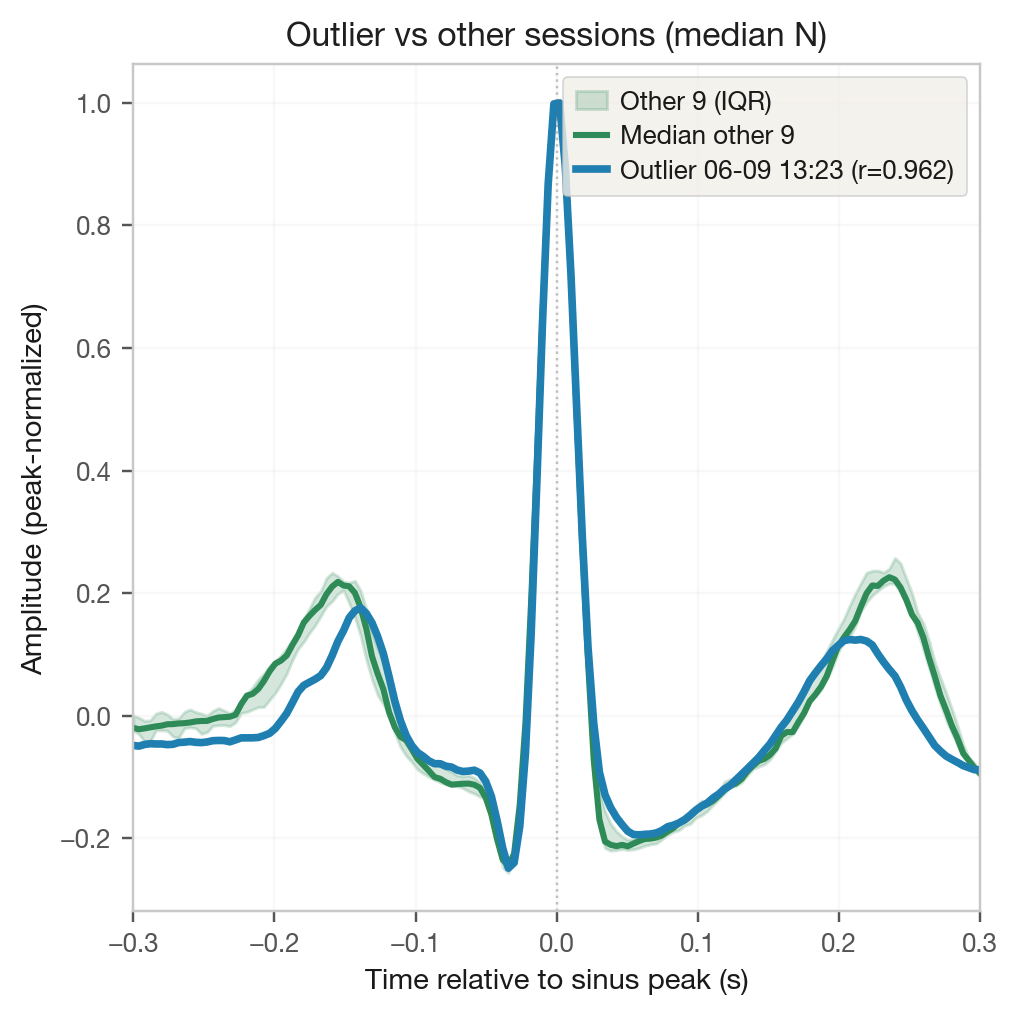
\includegraphics[width=0.58\linewidth]{05_n_outlier_comparison.png}
  \caption{Outlier session (seated, trunk-flexed) median N vs the median and IQR of the other nine sessions.}
\end{figure}
\tableOutlier

% ===================== 5. INTERP vs COMP =====================
\section{Interpolated vs compensated PVCs --- method \& validation}
Every PVC sits between a preceding and a following sinus beat (N--PVC--N).
\textbf{Conventionally} the two kinds are told apart by what happens to the
sinus node, measured R-to-R from QRS peak to QRS peak: an \interp{interpolated}
PVC slips in without resetting the SA node, so the next sinus beat stays on
schedule and N--PVC--N $\approx 1\times$ the sinus cycle; a \comp{compensated}
PVC resets the SA node, the next sinus beat is delayed by a full pause, and
N--PVC--N $\approx 2\times$.

\reportfig{06_interpolated_vs_compensated_example.png}{One PVC shown both ways: the conventional sum and the actual post-extrasystolic pause, against the locally-estimated sinus cycle.}

The reference sinus cycle is not a single session-wide number: this subject has
marked respiratory sinus arrhythmia, so it is estimated \textbf{locally} as the
median of the nearest N--N intervals around each PVC. A \textbf{prematurity
guard} discards beats whose coupling (\rrpre) is not shorter than that local
sinus cycle --- physically impossible for a true (premature) PVC, and a sign
that a small sub-threshold sinus beat was missed in the gap; 118 beats
($\approx$1\%) are set aside this way.

\subsection{Why the conventional sum leaves a grey zone --- and how the data resolves it}
Applying the strict sum rule ($1.85$--$2.15\times$ for a ``full'' pause) leaves
a wide band of beats in between. The data are cleaner than the rule suggests.
Two distributions: on the left the conventional \textbf{sum S}; on the right the
\textbf{actual pause \rrpost} after the PVC. Both are clearly \textbf{bimodal}
--- almost every beat falls into one lump or the other, with a near-empty valley
between them.

\reportfig{07_distributions_of_s_and_rr_post.png}{Distributions of the conventional sum S (left) and the actual pause RR\textsubscript{post} (right) --- both clearly bimodal.}

S and the pause agree on $\sim$99\% of beats but disagree on a few: the same S
can hide a short or a long pause depending on the coupling. When they disagree,
the variable that matches what is \textbf{seen on the trace and felt} is the
\textbf{pause} --- a long pause loads the ventricle and the next beat lands as a
forceful ``thump''. So the operative split is made on \rrpost{}, at the empirical
valley $\pauseValley\times$ the sinus cycle: shorter $\rightarrow$
\interp{interpolated} (silent), longer $\rightarrow$ \comp{compensated} (felt).
Across the dataset that gives \textbf{\pctInterp\% interpolated} and
\textbf{\pctComp\% compensated} on \methodBeats{} classified beats; only
$\sim$1\% sit within $\pm0.10$ of the valley (genuinely borderline), and those
that stay truly undecided are noise --- removed by exclusion / the guard rather
than forced into a class.

\subsection{How it looks on the trace}
The same classification on a continuous strip (session 2026-06-08 22:01): the
QRS of each PVC is \interp{blue} when interpolated (the sinus rhythm carries on
with no gap) and \comp{red} when compensated (a clear pause follows). This
two-way split is what the subject actually perceives: the interpolated beats
carry no pause and go unnoticed, the compensated ones are followed by the pause
and the potentiated beat felt as a \textbf{skipped / missed beat}.

\reportfig{08_final_2_class_strip.png}{The two-class split on a continuous strip: interpolated (blue) carry no pause, compensated (red) are followed by one.}

% ===================== 6. CROSS-SESSION =====================
\section{Cross-session rhythm \& burden dynamics}
Longitudinal comparison across all sessions, recomputed at every run.
\textbf{Burden} $=$ PVCs / all beats; \textbf{effective SA rate} $=$ 60000 /
median N--N interval (the rate a wrist pulse would read, since most PVCs are
non-perfusing).
\begin{itemize}
  \item \textbf{Burden by session} --- how the PVC load varies recording to recording.
  \item \textbf{Effective rate vs pause type} --- at lower SA rates interpolated
        (silent) beats tend to prevail; as the rate rises they shift toward
        compensated (felt) ones.
  \item \textbf{Composition} --- interpolated / compensated / incomplete share per session.
  \item \textbf{Coupling stability} --- a tight, session-stable pre-PVC coupling
        is consistent with a single monomorphic focus.
\end{itemize}

\reportfig{09_cross_session_rhythm_and_burden.png}{Cross-session burden, effective rate vs pause type, composition, and coupling stability.}
\tableCross

\textbf{Key pattern.} The single relationship that ties the dataset together:
the share of \comp{compensated} (felt) PVCs rises with the resting sinus rate
while \interp{interpolated} (silent) ones fall --- so the number of thumps the
subject notices tracks heart rate, not raw PVC count. Each point is one session;
curves are a weighted logistic fit, the trend quantified by Spearman's r in the
title.

\reportfig{10_resting_rate_vs_felt_pvcs.png}{Felt (compensated) PVC share rises with resting sinus rate while interpolated falls; each point is one session.}

% ===================== 7. SUMMARY TABLE =====================
\section{Per-session summary}
Every session as a column, every metric as a row, computed on the validated
definitions used throughout (local-sinus pause split, the couplet detector
below, real pre-PVC coupling median). ``Guarded'' $=$ PVCs whose pause was
unmeasurable (a sinus beat hidden in the gap), excluded from the interp/comp
split. ``AF score'' is the 0--4 atrial-fibrillation \emph{signal} screen
(RMSSD$>$100, pNN50$>$40, high RR entropy, unimodal $+$ high CV) --- a
signal-level check, not a diagnosis.

\tableSummary

% ===================== 8. PAUSE DISTRIBUTION =====================
\section{Per-session pause distribution}
One row per recording, using the validated criterion: each beat's pause \rrpost{}
measured against its \emph{local} sinus cycle, split at the global valley
($\pauseValley\times$). The left hump (\interp{blue, $\approx$0.7$\times$}) are
interpolated (silent) beats; the right hump (\comp{pink, $\approx$1.45$\times$})
compensated (felt) ones. A session whose mass sits almost entirely on one side
has a correspondingly lopsided \emph{perceived} burden --- the driver behind the
key pattern above.

\reportfig{11_per_session_pause_distribution.png}{Per-session pause distribution against the local sinus cycle, split at the global valley.}

% ===================== 9. COUPLING / SINGLE FOCUS =====================
\section{Per-session coupling distribution \& single-focus check}
\textbf{What the coupling interval is.} The coupling (\rrpre) is the time from
the preceding normal beat to the PVC --- how long after each sinus beat the
ectopic fires. A single focus re-entering on the same circuit fires at a
near-constant coupling, so a \textbf{tight, recording-to-recording-stable peak}
is the signature of one monomorphic focus; a \textbf{second focus} would add a
separate coupling peak \emph{with a different QRS shape}.

\textbf{Single-focus check (statistical).} For every session a 1- vs 2-component
Gaussian mixture is fit to the coupling; a session is flagged \emph{bimodal}
only when the two-component fit is genuinely two-peaked (a real trough, not mere
skew) and improves the BIC --- confirmed offline by a parametric-bootstrap
likelihood-ratio test ($p\approx0.002$). Result: \textbf{2 sessions} show a
genuinely bimodal coupling (06-05 18:29, 06-06 15:08); in each the two coupling
clusters have \emph{identical} QRS morphology, so this is the same monomorphic
focus discharging at two coupling intervals (coupling modulation), \emph{not} a
second focus. Sessions that show only a right-skewed shoulder rather than two separated
modes (for example 06-05 14:59) are deliberately left unflagged; forcing a split on them
anyway still yields two clusters with essentially identical QRS (template
$r\approx0.998$), so those tails belong to the same focus too. No session shows a
morphologically distinct second focus.

\reportfig{12_per_session_coupling_distribution.png}{Per-session coupling distribution with the statistical single-focus check.}

% ===================== 10. COUPLETS =====================
\section{Couplets --- detection, count \& overlay}
A \textbf{couplet} is two PVCs in a row (RR 200--700\,ms) that is \emph{not}
part of a longer run --- the simplest repetitive ectopy, worth counting because
frequency and uniformity speak to risk. \textbf{46 couplets across 7/10 sessions}
(none in 3). The inter-PVC interval is strikingly tight --- median 416\,ms
(range 384--464\,ms) --- and the two beats share the same morphology: the
couplets are uniform and consistent with the same single focus firing twice, not
a second focus or a malignant polymorphic pair.
\begin{itemize}
  \item \textbf{Count per session} (same session colours as above).
  \item \textbf{All couplets overlaid}, each aligned on the first PVC's peak and
        amplitude-normalised --- if they stack, they are uniform.
  \item \textbf{First vs second beat}: median QRS of the first PVC (\interp{blue})
        against the second (\textcolor{Orange}{orange}). High correlation means
        both beats come from the same focus.
\end{itemize}

\reportfig{13_couplets_count_and_overlay.png}{Couplet count per session, all couplets overlaid, and first-vs-second-beat median QRS.}

A few couplets in their raw recording context ($\pm$5\,s), same format as the
example strips earlier --- green trace, the two ectopic QRS in \comp{red}. One
clean representative is shown per \textbf{distinct local rhythm} (the N/V motif
printed in each title) so the gallery spans the variations.

\reportfig{14_couplet_example_strips.png}{A few couplets in raw context ($\pm$5\,s), one per distinct local rhythm motif.}

\subsection{Local rhythm motif --- does the couplet sit in a repeating pattern?}
Coding each beat as N (sinus) or V (PVC) for the four beats before and after
every couplet reveals whether it recurs inside a fixed rhythm. The couplet is
usually embedded in one recurring rhythm: the motif
\texttt{N V N N [V V] N V N N} occurs in \textbf{30/46 (65\%)} of couplets --- an
organised, trigeminy-like cadence (an isolated PVC, two sinus beats, the
couplet, then the same again). These 30 occurrences are spread across six of the
recordings, with no single session contributing more than a third, so the cadence is a
stable trait of the focus rather than a quirk of one day. It is not universal: the remaining 16 show
variants (the couplet out of a longer sinus run, after a bigeminal stretch, or
followed by quiet), which is why the example strips span different motifs rather
than repeating the dominant one.

\reportfig[0.82\linewidth]{15_couplet_local_rhythm_motifs.png}{Local rhythm motifs around the couplet.}

% ===================== 11. RESPIRATION =====================
\section{Respiration (EDR) \& respiratory-phase trigger}\label{sec:edr}
The final question: are the PVCs tied to \textbf{breathing}? There is no
respiration belt, but the breath leaves a fingerprint on the ECG --- chest
movement and lung-impedance change make the R-wave amplitude rise and fall with
each breath (ECG-derived respiration, \textbf{EDR}). Recovering that signal from
the R-amplitude of the normal beats (cubic-resampled to 4\,Hz, band-passed
0.1--0.5\,Hz, instantaneous phase by Hilbert transform) lets us ask, for every
beat, \emph{where in the breath} it fell.

Respiration was recovered in \textbf{10/10} sessions; PVC timing is
significantly coupled to respiratory phase in \textbf{10/10} of them ($\chi^2$
across phase bins, $p<0.05$) --- so yes, there is a real correlation. The
R-amplitude is largest at \textbf{full lungs} (the subject confirmed this
directly while recording), so the phase peak sits at full inflation /
end-inspiration: PVCs are over-represented there (mean peak $\times2.6$ vs
chance) and sparsest near empty lungs. That points to a mechanical, lung-volume
/ cardiac-filling trigger at peak inflation (diaphragm lowest, maximal venous
return and chamber stretch) --- rather than the end-expiratory vagal one
previously assumed.

\reportfig{16_edr_respiration_demo.png}{ECG-derived respiration: the R-amplitude of sinus beats traces the breath; PVCs land on a recurring part of it.}

Below: the phase distribution of all PVCs vs normal beats (polar) and the
per-session enrichment around the respiratory cycle (values above $\times1$ mark
phases where PVCs are over-represented). Phase 0/100\% is \textbf{full lungs}
(largest R-amplitude, end-inspiration); 50\% is empty lungs (end-expiration).
The enrichment peaks at full lungs.

\reportfig{17_respiratory_phase_vs_pvc_enrichment.png}{Phase distribution of all PVCs vs normal beats (polar) and per-session enrichment around the respiratory cycle.}

\subsection{Respiratory phase by PVC type}
Do the different PVC types fall at the same point in the breath? This rosette
splits the PVCs by type --- \interp{interpolated}, \comp{compensated} and
\coupled{coupled} (both beats of each couplet) --- with each type's phase
density normalised so the \emph{shape} is comparable despite very different
counts. The phase peaks are interpolated 79\%, compensated 12\%, coupled 87\%
(\% of cycle, $0=$ full lungs): all three favour roughly the same phase near
full lungs, so they share one respiratory trigger and do not pick out separate
phases.

\reportfig[0.6\linewidth]{18_respiratory_phase_by_pvc_type.png}{Respiratory phase by PVC type --- interpolated, compensated and coupled all peak near full lungs.}

\tableResp

A significant $p$ means the PVCs are \textbf{not} uniformly spread across the
breath --- they cluster at a phase, i.e.\ respiration modulates the focus. This
is a signal-level observation, not a clinical finding.

% ===================== COLOPHON =====================
\vfill
{\footnotesize\color{muted}
\textbf{About this document.} Sample rate 250 Hz, single precordial lead
(AD8232), 1st-order IIR bandpass 0.3--25 Hz, QRS detector and PVC classifier as
in the setup box. Sessions filtered: size $\geq$ 5 MB and $\geq$ 50 PVCs. It is
a personal-use, educational notebook and a discussion document for the
supervising cardiologist --- it does \textbf{not} constitute a diagnostic
report.\par
\vspace{0.4em}
This report was built with heavy AI assistance; some of its analyses were
initially wrong and were caught only by ground-truth checks (notably the
respiratory phase, which was first concluded backwards). That story --- what it
teaches about trusting AI with biomedical data --- is written up in
\texttt{docs/caso-studio-ai-sicurezza.md}.\par}

\end{document}
